%
% windschief.tex
%
% (c) 2018 Prof Dr Andreas Müller, Hochschule Rapperswil
%
\documentclass[tikz]{standalone}
\usepackage{times}
\usepackage{amsmath}
\usepackage{txfonts}
\usepackage[utf8]{inputenc}
\usepackage{graphics}
\usetikzlibrary{arrows,intersections,math}
\usepackage{ifthen}
\begin{document}

\newboolean{showgrid}
\setboolean{showgrid}{false}

\begin{tikzpicture}[>=latex,thick]

% Povray Bild
\node at (0,0) {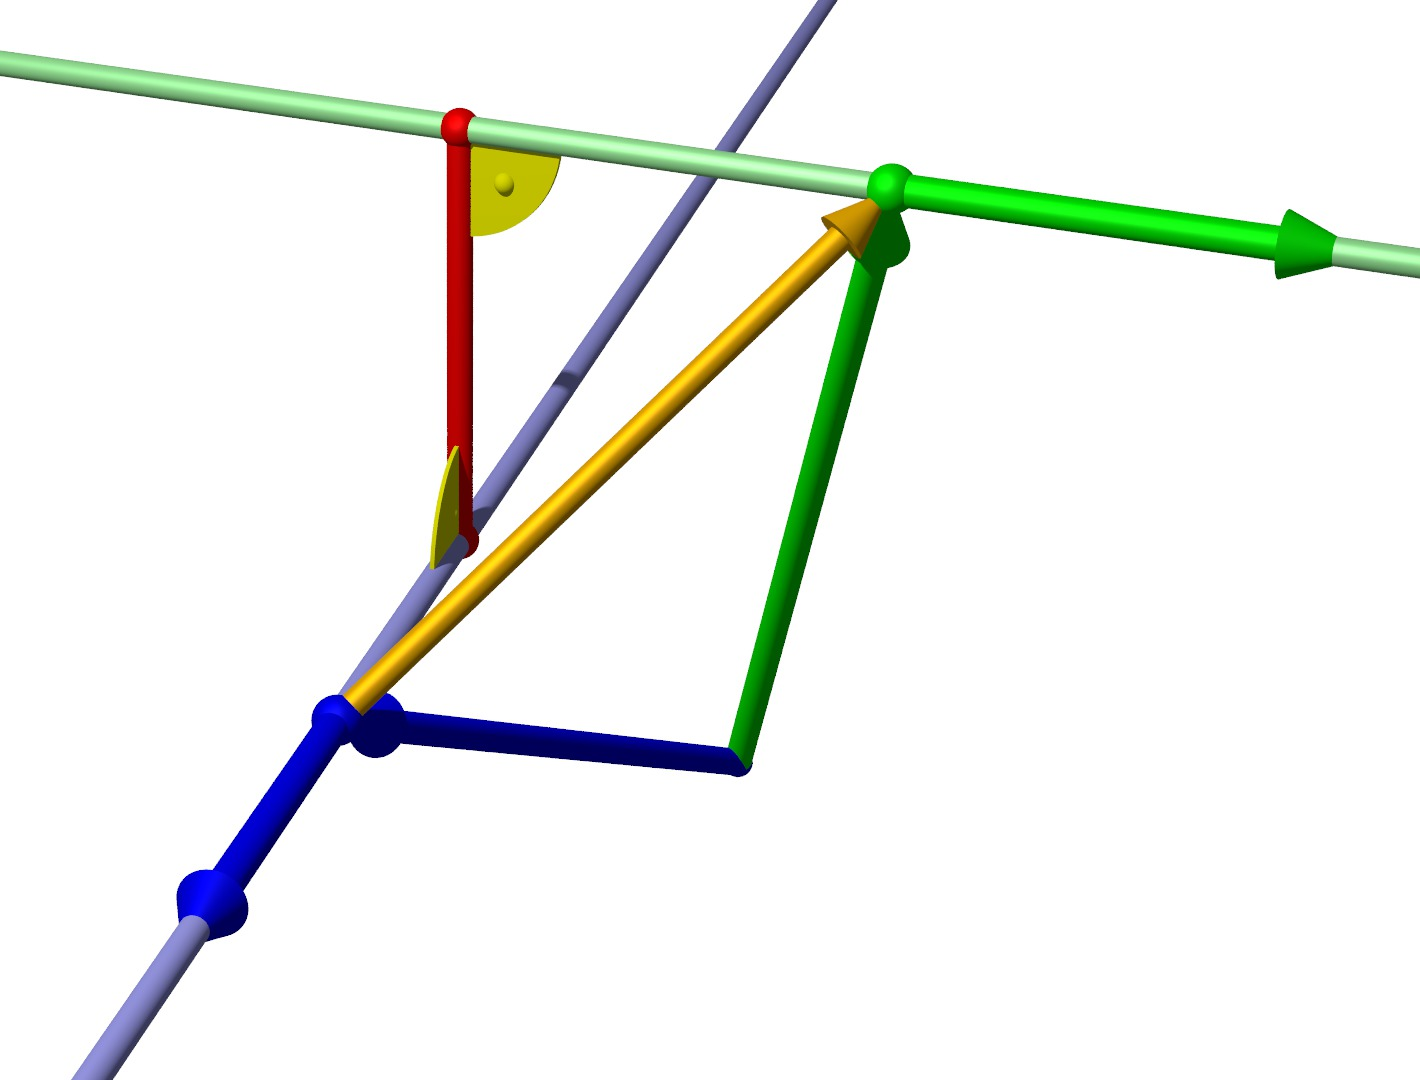
\includegraphics[width=12cm]{windschief.jpg}};

% Gitter
\ifthenelse{\boolean{showgrid}}{
\draw[step=0.1,line width=0.1pt] (-6,-6) grid (6, 6);
\draw[step=0.5,line width=0.4pt] (-6,-6) grid (6, 6);
\draw (-6,-6) grid (6, 6);
\fill (0,0) circle[radius=0.05];
}{}

% Nullpunkt
\node at (0.5,-2.2) {$O$};

% Gerade g1
\node at (1.5,3.5) {$P_1$};
\node at (5,3) {$\vec{r}_1$};
\node at (-5,4.3) {$g_1$};
\node at (1.6,1.8) {$\vec{p}_1$};

% Gerade g0
\node at (-3.6,-1.2) {$P_0$};
\node at (-4.5,-2.5) {$\vec{r}_0$};
\node at (-5.4,-4) {$g_0$};
\node at (-2.3,-2.0) {$\vec{p}_0$};

% Differenz
\node at (-0.6,0.0) {$\vec{p}_1-\vec{p}_0$};

% Abstand
\node at (-2.3,1.7) [left] {$d\,\|\, \vec{n} = \vec{r}_0\times\vec{r}_1$};

\end{tikzpicture}

\end{document}

